\documentclass{article}
\usepackage{mathrsfs} % for scripts
\usepackage{standalone}
\usepackage{tikz}
\usetikzlibrary{arrows}
\usetikzlibrary{hobby}
\begin{document}
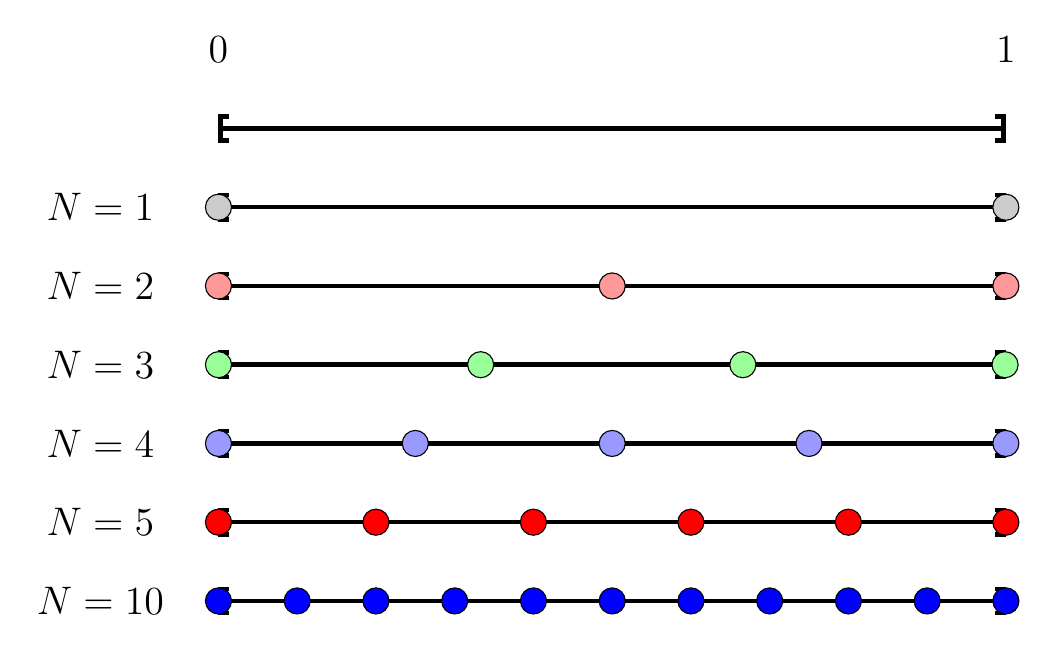
\begin{tikzpicture}[scale=10,darkstyle/.style={circle,draw,fill=gray!40,minimum size=01}]
    \begin{scope}
	\draw[{[-]}, ultra thick] (0,0) -- (1,0);
	\node at (0,0.1) {\Large$0$};
	\node at (1,0.1) {\Large$1$};
    \end{scope}
    \begin{scope}[yshift=-0.1cm]
	\node at (-0.15,0) {\Large$N=1$};
	\draw[{[-]}, ultra thick] (0,0) -- (1,0);
	\foreach \x in {0,...,1}
	 \node [darkstyle]  (\x 0) at (\x,0) {}; 
     \end{scope}
     \begin{scope}[yshift=-0.2cm]
	\node at (-0.15,0) {\Large$N=2$};
	\draw[{[-]}, ultra thick] (0,0) -- (1,0);
	 \foreach \x in {0,...,2}
	  \node [circle,draw,fill=red!40,minimum size=0.5]  (\x 0) at (0.5*\x,0) {}; 
      \end{scope}
      \begin{scope}[yshift=-0.3cm]
	\node at (-0.15,0) {\Large$N=3$};
	\draw[{[-]}, ultra thick] (0,0) -- (1,0);
	 \foreach \x in {0,...,3}
	  \node [circle,draw,fill=green!40,minimum size=0.5]  (\x 0) at (0.333*\x,0) {}; 
    \end{scope}
    \begin{scope}[yshift=-0.4cm]
	\node at (-0.15,0) {\Large$N=4$};
	\draw[{[-]}, ultra thick] (0,0) -- (1,0);
	\foreach \x in {0,...,4}
	\node [circle,draw,fill=blue!40,minimum size=0.5]  (\x 0) at (0.25*\x,0) {}; 
    \end{scope}
    \begin{scope}[yshift=-0.5cm]
	\node at (-0.15,0) {\Large$N=5$};
	\draw[{[-]}, ultra thick] (0,0) -- (1,0);
	\foreach \x in {0,...,5}
	\node [circle,draw,fill=red,minimum size=0.5]  (\x 0) at (0.2*\x,0) {}; 
    \end{scope}
    \begin{scope}[yshift=-0.6cm]
	\node at (-0.15,0) {\Large$N=10$};
	\draw[{[-]}, ultra thick] (0,0) -- (1,0);
	\foreach \x in {0,...,10}
	\node [circle,draw,fill=blue,minimum size=0.5]  (\x 0) at (0.1*\x,0) {}; 
    \end{scope}
\end{tikzpicture}
\end{document}
